%--------------------------------------
% Create title frame
\titleframe

%--------------------------------------
% Table of contents
\begin{frame}{Overview}
  \setbeamertemplate{section in toc}[sections numbered]
  \tableofcontents[hideallsubsections]
\end{frame}


\begin{frame}
  \frametitle{For more info}

Short intro in my PhD thesis: \url{https://orbi.uliege.be/handle/2268/82167}

An introductory course: \url{https://people.montefiore.uliege.be/lwh/AIA/}


\end{frame}
\section{Introduction and categories of Machine Learning problems}
\begin{frame}{Machine Learning}
  
  Machine learning is the field of computer algorithms that improve automatically through experience and data.
  Common applications:
      \begin{itemize}
        \item Image recognition
        \item Email Spam \& Malware filtering
        \item Speech recognition
        \item Social media customized advertising
        \item Netflix's recommendations
        \item Medical diagnosis
      \end{itemize}
\end{frame}

\begin{frame}{Machine Learning, why now?}
      \begin{itemize}
        \item More Data
        \item Faster compute engines
        \item Algorithms (old and new)
        \item Machine learning software
      \end{itemize}
  
\end{frame}


\begin{frame}{Categories of Machine Learning problems}
  \begin{itemize}
    \item Supervised Learning
    \item Unsupervised Learning
    \item Reinforcement Learning
    \item And many variants ...
  \end{itemize}
\end{frame}

\begin{frame}[allowframebreaks]{Supervised Learning}
  \begin{itemize}
    \item Starting point:  a dataset where inputs and outputs are clearly identified, e.g.:
    \begin{center}
      \begin{tabular}{*{4}{c} c}
        \toprule
        \multicolumn{4}{c}{Inputs} & Output \\
        $X_1$ & $X_2$ & $X_3$ & $X_4$ & $Y$  \\
        \midrule
        -0.61 & -0.43 & Y & 0.51 & Healthy \\
        -2.3 & -1.2 & N & -0.21 & Disease \\
        0.33 & -0.16 & N & 0.3 & Healthy \\
        0.23 & -0.87 & Y & 0.09 & Disease \\
        -0.69 & 0.65 & N & 0.58 & Healthy \\
        0.61 & 0.92 & Y & 0.02 & Disease \\
        \bottomrule
      \end{tabular}
    \end{center}
    \item Goal: find a function $f_{\Theta}$ of the inputs that approximates at best the outputs, e.g.
    $$\hat{y} = f(x_1,x_2,x_3,x_4 )$$ 
    \item \textcolor{blue}{Training set}: part of the available data used for identifying the best possible function $f_{\Theta^\star}$ (its best parameters), \textcolor{red}{Test set}: part of the dataset to evaluate $f$.
    \begin{center}
      \begin{tabular}{*{4}{c} c}
        \toprule
        %\multicolumn{4}{c}{Inputs} & Output \\
        $X_1$ & $X_2$ & $X_3$ & $X_4$ & $Y$  \\
        \midrule
        \rowcolor{blue!20} -0.61 & -0.43 & Y & 0.51 & Healthy \\
        \rowcolor{blue!20} -2.3 & -1.2 & N & -0.21 & Disease \\
        \rowcolor{blue!20} 0.33 & -0.16 & N & 0.3 & Healthy \\
        \rowcolor{blue!20} 0.23 & -0.87 & Y & 0.09 & Disease \\
        \rowcolor{red!20} -0.69 & 0.65 & N & 0.58 & Healthy \\
        \rowcolor{red!20} 0.61 & 0.92 & Y & 0.02 & Disease \\
        \bottomrule
      \end{tabular}
    \end{center}
    \item Inference: When $f$ is determined, do a prediction using $f$ for inputs when the output is not available
    \begin{center}
      \begin{tabular}{*{4}{c} c}
        \toprule
        
        $X_1$ & $X_2$ & $X_3$ & $X_4$ & $Y$  \\
        \midrule
        0.75 & 0.49 & Y & -0.88 & \textcolor{blue}{$f(0.75, 0.49, Y, -0.88)$} \\
        \bottomrule
        \end{tabular}
    \end{center}
  \end{itemize}

\end{frame}

\begin{frame}[allowframebreaks]{Unsupervised Learning}
  \begin{columns}
    \begin{column}{0.5\textwidth}
  \begin{itemize}
    \item Unsupervised learning does not use labeled data. 
    \item Instead of making predictions, the goal of unsupervised learning is to find the underlying structure of dataset and group that data according to similarities.
    \item Example: Clustering. Assuming we have a dataset of points in a 2D space, group them in 3 clusters:
  \end{itemize}

\end{column}
\begin{column}{0.5\textwidth}
  \begin{center}
    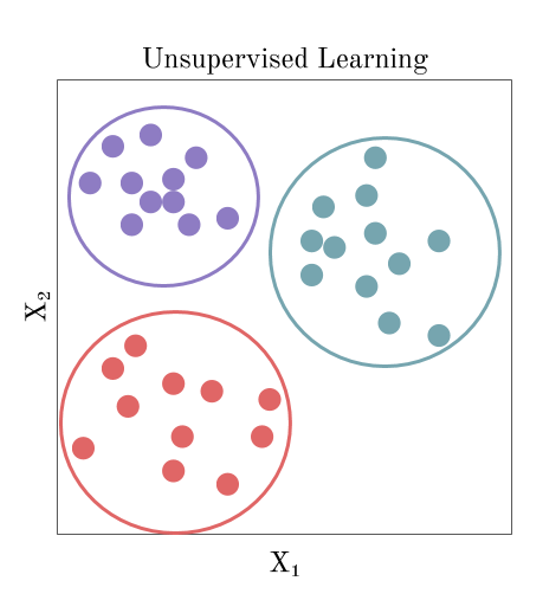
\includegraphics[width=0.8\textwidth]{images/clustering.png}
  \end{center}
\end{column}
\end{columns}
Application: if you have 365 days of conmumption data with 15 minute resolution, identify e.g. a subset of 12 days that represent well the 365 days.
\end{frame}

\begin{frame}{Reinforcement Learning}
  \begin{columns}
    \begin{column}{0.6\textwidth}
  \begin{itemize}
    \item Learning from interactions with an environment.
    \item Goal: By interacting with and environment, learn to take actions in any given state to maximize a reward function.
    \item Example:
      \begin{itemize}
        \item State: Robot position in a labyrinth.
        \item Actions: Go ahead, turn right, turn left.
        \item Reward: Get a reward each time the robot gets out.
        \item Goal: Learn how to get out as fast as possible.
      \end{itemize}
  \end{itemize}
\end{column}
\begin{column}{0.4\textwidth}

  \begin{center}
    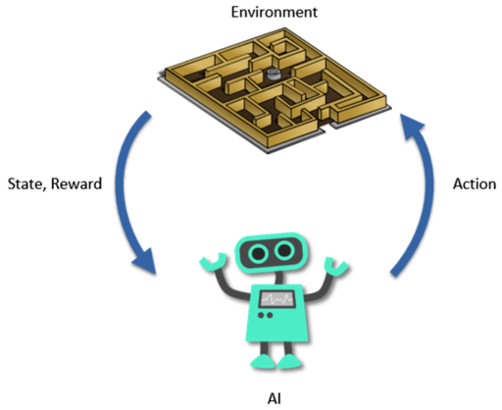
\includegraphics[width=0.9\textwidth]{images/RL.png}
  \end{center}

\end{column}
\end{columns}
\end{frame}

\section{Supervised Learning}

\begin{frame}{Supervised Learning (SL)}
  \begin{itemize}
    \item Data organized as a set of $N$ objects described by input features and output labels.
    $$\{(x_1, y_1), (x_2, y_2), \dots, (x_N, y_N)\} $$
    \item Features $x_i$ are easily obtained by observation.
    \item Output $y_i$ is provided by an expert or is the result of difficult/costly observation/computation.
  \end{itemize}
\end{frame}

\begin{frame}{Mapping, Loss Function, Expected Loss}
  \begin{itemize}
    \item SL algorithms search for a mapping $f : \mathcal{X} \rightarrow \mathcal{Y}$ between feature and output spaces that generalizes well to elements for which the output value has not been observed.
    \item Define a loss function $$ L: \mathcal{Y} \times \mathcal{Y}  \rightarrow \mathbb{R}_+$$
    \item Search for $f$ which minimizes the expected loss:
      \[ \mathbb{E}_{\mathbb{P}_{X,Y}}[L(y, f(x))] \]
  \end{itemize}
\end{frame}

\begin{frame}{Classification and Regression}
  
  \begin{columns}
    \begin{column}{.5\textwidth}
    
    Classification:
    \begin{itemize}
      \item Approximate a mapping $f$ from inputs $X$ to \textbf{discrete} outputs $y$.
      \item Examples: Spam detection, room occupancy.
    \end{itemize}
      \begin{center}
        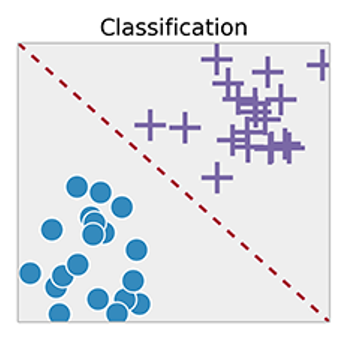
\includegraphics[width=0.5\textwidth]{images/classification.png}
      \end{center}
    \end{column}  
    \begin{column}{.5\textwidth}
    Regression:
    \begin{itemize}
      \item Approximate a mapping $f$ from inputs $X$ to \textbf{continuous} outputs $y$.
      \item Examples: House price prediction, time series forecasting.
    \end{itemize}
    \begin{center}
      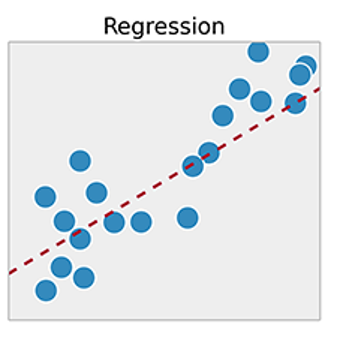
\includegraphics[width=0.5\textwidth]{images/regression.png}
    \end{center}
    \end{column}
  \end{columns}
\end{frame}

\begin{frame}{Empirical Loss Minimization}
  \begin{itemize}
    \item We usually don't know the joint distribution.
    \item Instead, minimize an estimate of the expected loss, the \textbf{empirical loss}:
      \[ \frac{1}{N} \sum_{i=1}^{N} L(y_i, f(x_i)) \]
  \end{itemize}
\end{frame}

\begin{frame}{Model Selection}
  \begin{itemize}
    \item By selecting a supervised learning method\footnote{See page \ref{SL_methods}.} (kNN, SVM, etc.), we restrict and parameterize the hypothesis space of functions $f_\Theta(x)$
    \item But how do we pick up a method / model, and how do we optimize its parameters? \textit{The next example will give us some insights.}
  \end{itemize}
\end{frame}


\begin{frame}{Linear Model}
  \begin{columns}
    \begin{column}{0.5\textwidth}
      \begin{itemize}
        \item Polynomial of degree 1 regression model with 1 input and 1 output.
        \item Equation: $f(X) = \omega_0 + \omega_1 X$ 
        \item Learning phase: Find values for $\omega_0$ and $\omega_1$ to best fit the training set. 
      \end{itemize}
    \end{column}
    \begin{column}{0.5\textwidth}
      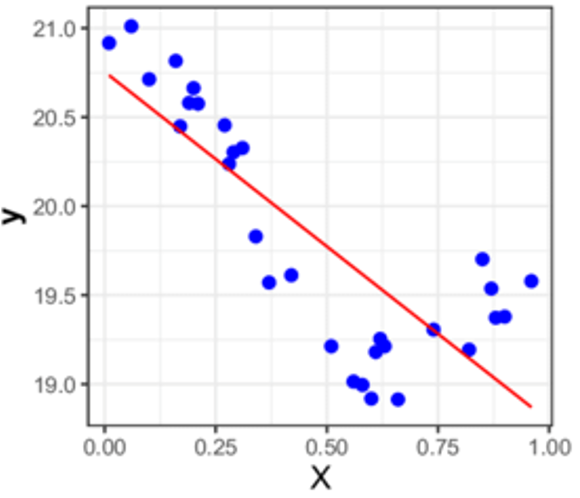
\includegraphics[width=0.8\textwidth]{images/lm.png}
    \end{column}
  \end{columns}
\end{frame}

\begin{frame}{Polynomial of degree 4}
  \begin{columns}
    \begin{column}{0.5\textwidth}
  \begin{itemize}
    \item Polynomial of degree 4 regression model with 1 input and 1 output
    \item Equation: $f(X) = \omega_0 + \omega_1 X + \omega_2 X^2 + \omega_3 X^3 + \omega_4 X^4$
    \item Learning phase: Find values for $\omega_0$, $\omega_1$, $\omega_2$, $\omega_3$, $\omega_4$ to best fit the training set.
  \end{itemize}
\end{column}
\begin{column}{0.5\textwidth}
  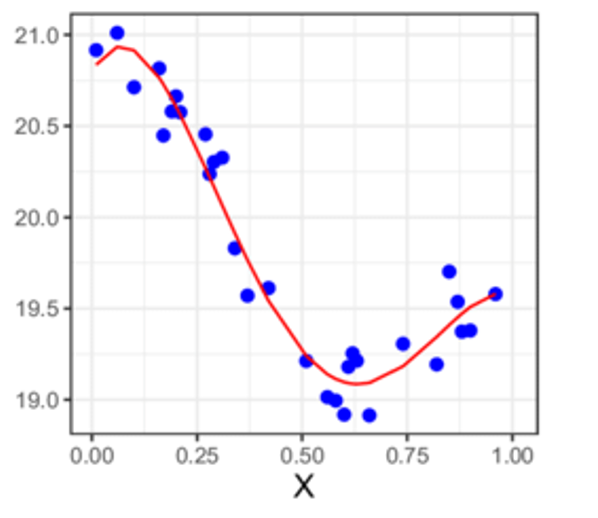
\includegraphics[width=0.8\textwidth]{images/pm4.png}
\end{column}
\end{columns}
\end{frame}

\begin{frame}{Polynomial of degree 20}
  \begin{columns}
    \begin{column}{0.5\textwidth}
  \begin{itemize}
    \item Polynomial of degree 20 regression model with 1 input and 1 output.
    \item Equation: $f(X) = \sum_{i=0}^{20} \omega_i X^i$
    \item Learning phase: Find values for $\omega_0, \dots, \omega_{20}$ to best fit the training set.
  \end{itemize}
\end{column}
\begin{column}{0.5\textwidth}
  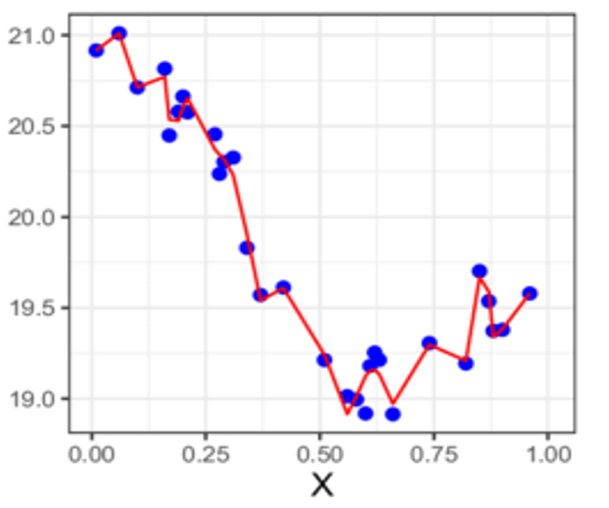
\includegraphics[width=0.8\textwidth]{images/pm20.png}
\end{column}
\end{columns}
\end{frame}

\begin{frame} {Model Selection}
  \begin{columns}
    \begin{column}{0.5\textwidth}
    Error\footnote{E.g. mean absolute error, see page \ref{regression_metrics}.} on the \alert{training set}
      \begin{itemize}
    \item Linear model: $0.4$
    \item Degree 4 polynomial: $0.14$
    \item Degree 20 polynomial model: $0.07$
  \end{itemize}
  \vspace{1cm}
  You need to evaluate your model on unseen data $\rightarrow$  \alert{Test set}
\end{column}
\pause
\begin{column}{0.5\textwidth}
  Error on the test set: 
  \begin{itemize}
    \item Linear model: $0.42$
    \item Degree 4 polynomial: $0.17$
    \item Degree 20 polynomial model: $2$
  \end{itemize}
  \vspace{1cm}
  Linear model is \alert{underfitting} while degree 20 polynomial is \alert{overfitting}, the best fit for this problem is the degree 4 polynomial. 
\end{column}
\end{columns}
\end{frame}


\begin{frame}{Overfitting and underfitting}
\begin{columns}
    \begin{column}{0.4\textwidth}
We can consider that data is composed of:
\begin{itemize}
  \item A main signal 
  \item A noise signal
\end{itemize}
\end{column}
\begin{column}{0.6\textwidth}
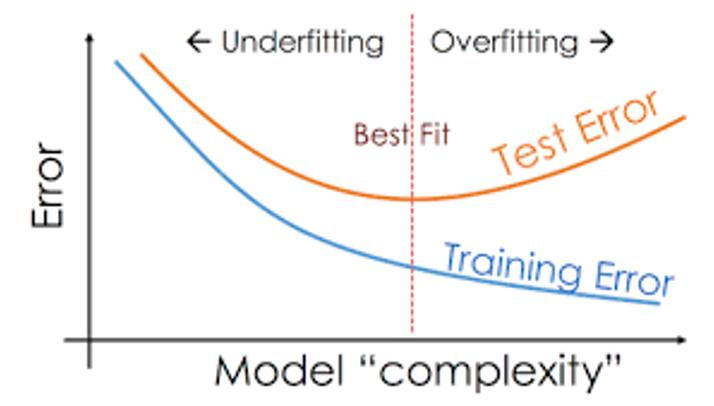
\includegraphics[width=0.8\textwidth]{images/under_and_over_fitting.png}
\end{column}
\end{columns}

\begin{itemize}
  \item Overfitting happens when the model captures the noise along with the main signal in data. (Degree 20 polynomial)
  \item Underfitting happens when a model is unable to capture the main signal in data. (Linear model)
\end{itemize}
\end{frame}

\begin{frame}[allowframebreaks]{Cross-validation}
  In general, adjusting your model based on your test set performance is bad practice. Cross-validation is a way to prevent overfitting without evaluating a model on the test set. 
  \begin{itemize}
    \item Split your initial training data into k subsets. 
    \item Iteratively train the algorithm on k-1 subsets while using the remaining fold as the “test” set (called validation set) to calculate the prediction error.
    \item Report the mean error over the k subsets. 
    \item Cross-validation allows you to tune hyperparameters with only your original training set. This allows you to keep your test set as a truly unseen dataset for selecting your final model.
  \end{itemize}
  
  \begin{center}
  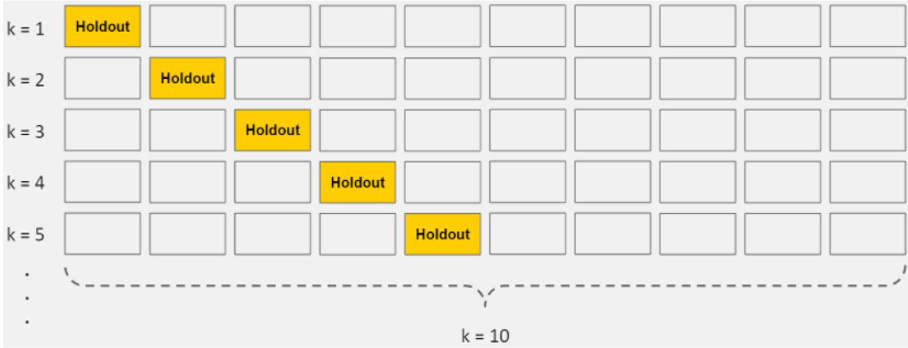
\includegraphics[width=0.8\textwidth]{images/CV.png}
  \end{center}
  \end{frame}

  \section{Supervised Learning Methods}

  \begin{frame}{There are many SL methods}
    \label{SL_methods}      
    \begin{itemize}
        \item (Linear) regression
        \item Nearest neighbors
        \item Regression and decision trees
        \item Support vector machines / support vector regression
        \item Artificial neural networks $\implies$ deep learning
        \item Ensemble methods
        \item …
    \end{itemize}
  \end{frame}
  
  \begin{frame}{$k$-NN}
    \begin{columns}
      \begin{column}{0.4\textwidth}  
      \begin{itemize}
          \item Find the $k$ nearest neighbors with respect to Euclidean distance.
          \item Output the most frequent class (classification) or the average outputs (regression) among the $k$ neighbors.
      \end{itemize}
      \end{column}
      \begin{column}{0.6\textwidth}
        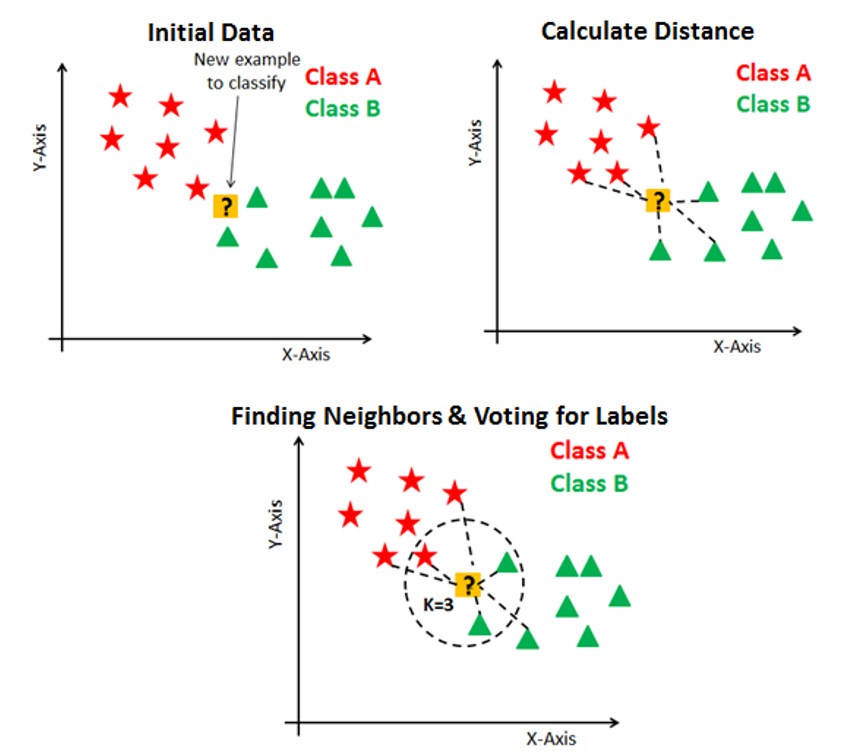
\includegraphics[width=0.9\textwidth]{images/knn.png}
      \end{column}
    \end{columns}
  \end{frame}

\subsection{Decision Trees}

\begin{frame}{Decision Tree}
  \begin{columns}
    \begin{column}{0.4\textwidth}  
  \begin{itemize}
    \item Choose the input that best separates the training set.
    \item Split the training set according to the chosen input.
    \item Proceed recursively until each object is correctly classified.
  \end{itemize}
\end{column}
\begin{column}{0.6\textwidth}
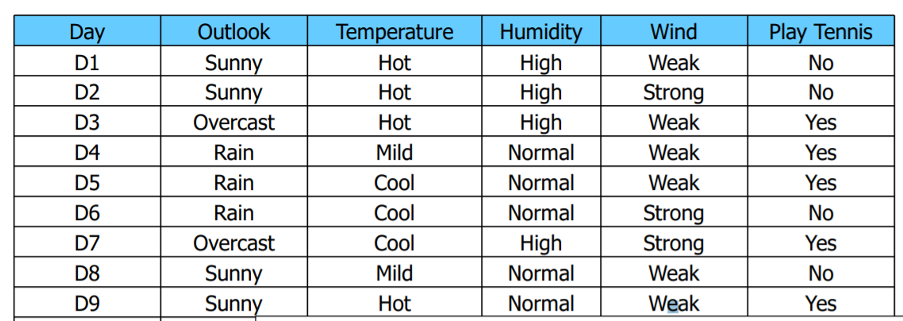
\includegraphics[width=0.9\textwidth]{images/DT1_1.png}\\
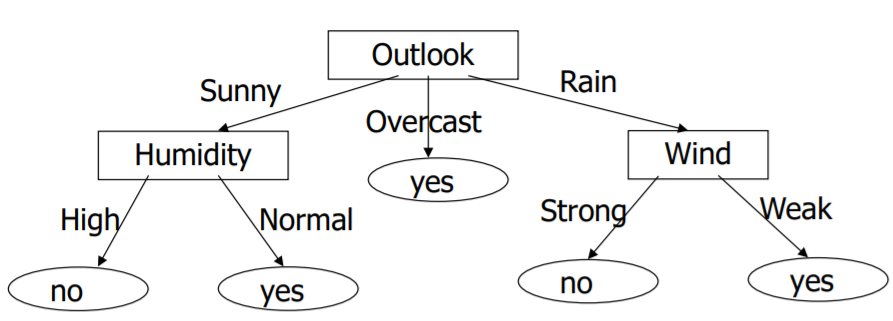
\includegraphics[width=0.8\textwidth]{images/DT1_2.png}
\end{column}
\end{columns}
\end{frame}

\begin{frame}
  \frametitle{Regression tree with 2 real features and one output}
  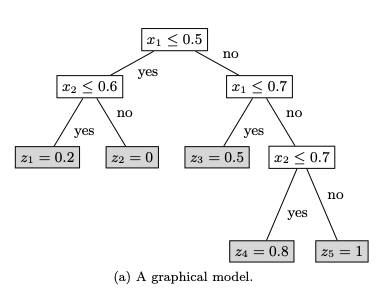
\includegraphics[width=0.45\textwidth]{images/RT_1.png}
  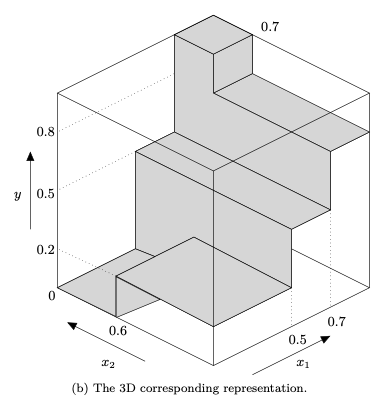
\includegraphics[width=0.45\textwidth]{images/RT_2.png}
\end{frame}

\begin{frame}{Top-down induction of a regression tree (TDIRT).}

  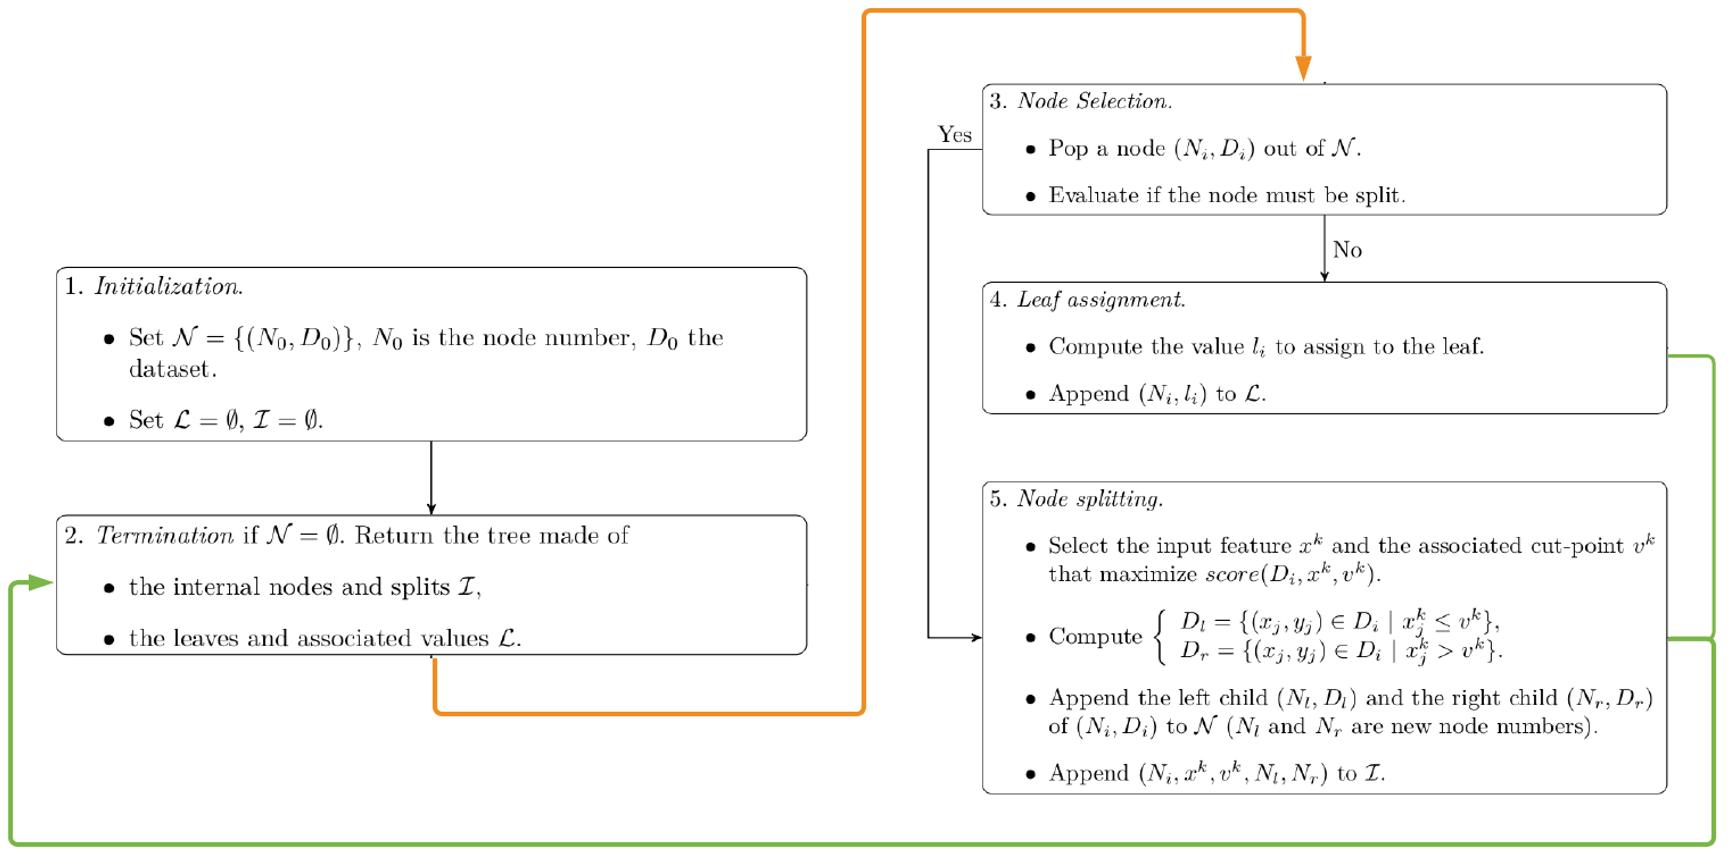
\includegraphics[width=0.95\textwidth]{images/TDIDT.png}


\end{frame}
\begin{frame}{Decision Tree Comments}
    \begin{itemize}
        \item If we use the mean squared error (MSE) criterion to estimate the accuracy of the tree predictor, defining $l_i$ (step 4) as the mean value of the outputs of the objects constituting a leaf $i$ is optimal with respect to empirical prediction error.
        \item To \alert{split} a node $i$ (step 5) , a test is defined by a feature $x_k$ and a cut-off value $v_k$.
        \item All the objects satisfying the test $x_k > v_k$ are assigned to the right successor node and the remaining ones are assigned to the left successor node.
    \end{itemize}
\end{frame}

\begin{frame}{Splitting Score}
    \begin{itemize}
        \item To find the best test, a score is computed for every input feature and for every possible cut-off value.
        \item For regression trees, a typical score measure is the relative decrease of output variance in the two successor nodes with respect to the output variance of the current node.
        $$score(D_i, x^k, v^k) = \frac{var\{y|D_i\} - \frac{|D_l|}{|D_i|} var\{y|D_l\} - \frac{|D_r|}{|D_i|} var\{y|D_r\}}{var\{y|D_i\}}$$
        \item The test with the highest variance reduction is chosen. 
    \end{itemize}
\end{frame}

\begin{frame}{Until When Do We Split?}
    \begin{itemize}
        \item It is more complicated to assess if a node should be split, i.e., to mitigate the complexity of the model.
        \item A classical way is to stop splitting when the number of objects in a node is below a threshold value.
        \item Many other techniques have been developed to identify the tree of optimal complexity (pruning methods).
    \end{itemize}
\end{frame}


\section{Steps to apply machine learning}

\begin{frame}{Steps to solve a supervised learning problem}

  \begin{enumerate}
    \item Collect and clean the data
    \item Select a suitable model
    \item Fit your model on the training set 
    \item Evaluate it on a validation set
    \item Adjust and improve your model (Overfitting? Underfitting?)
    \item \textit{Repeat steps 3-5 until you are satisfied}
    \item Evaluate your model on the test set
  \end{enumerate}
\end{frame}

\begin{frame}{1. Data collection and cleaning}
  \begin{itemize}
    \item Quantity: the more, the better
    \item Quality: Check if the data is well distributed
    \item Data rescaling (faster learning)
    \item Check missing values, wrong labeling, bad encoding
    \item Feature engineering     
  \end{itemize}
\end{frame}


\begin{frame}[allowframebreaks]{Hyperparameter tuning}

Example: K-nn model
Which number of neighbors k to choose ?
\begin{center}
  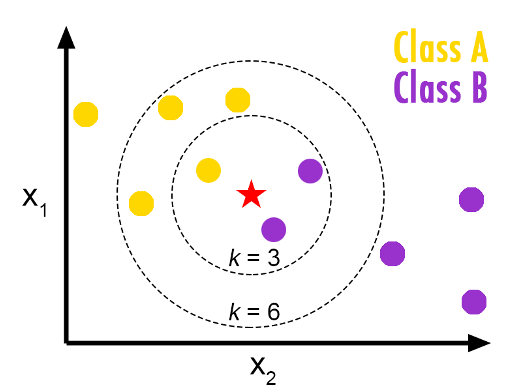
\includegraphics[width=0.4\textwidth]{images/model_selection_knn_1.png}
\end{center}
Use cross validation: try several values and pick the one that generalizes the best on the validation set
\begin{center}
  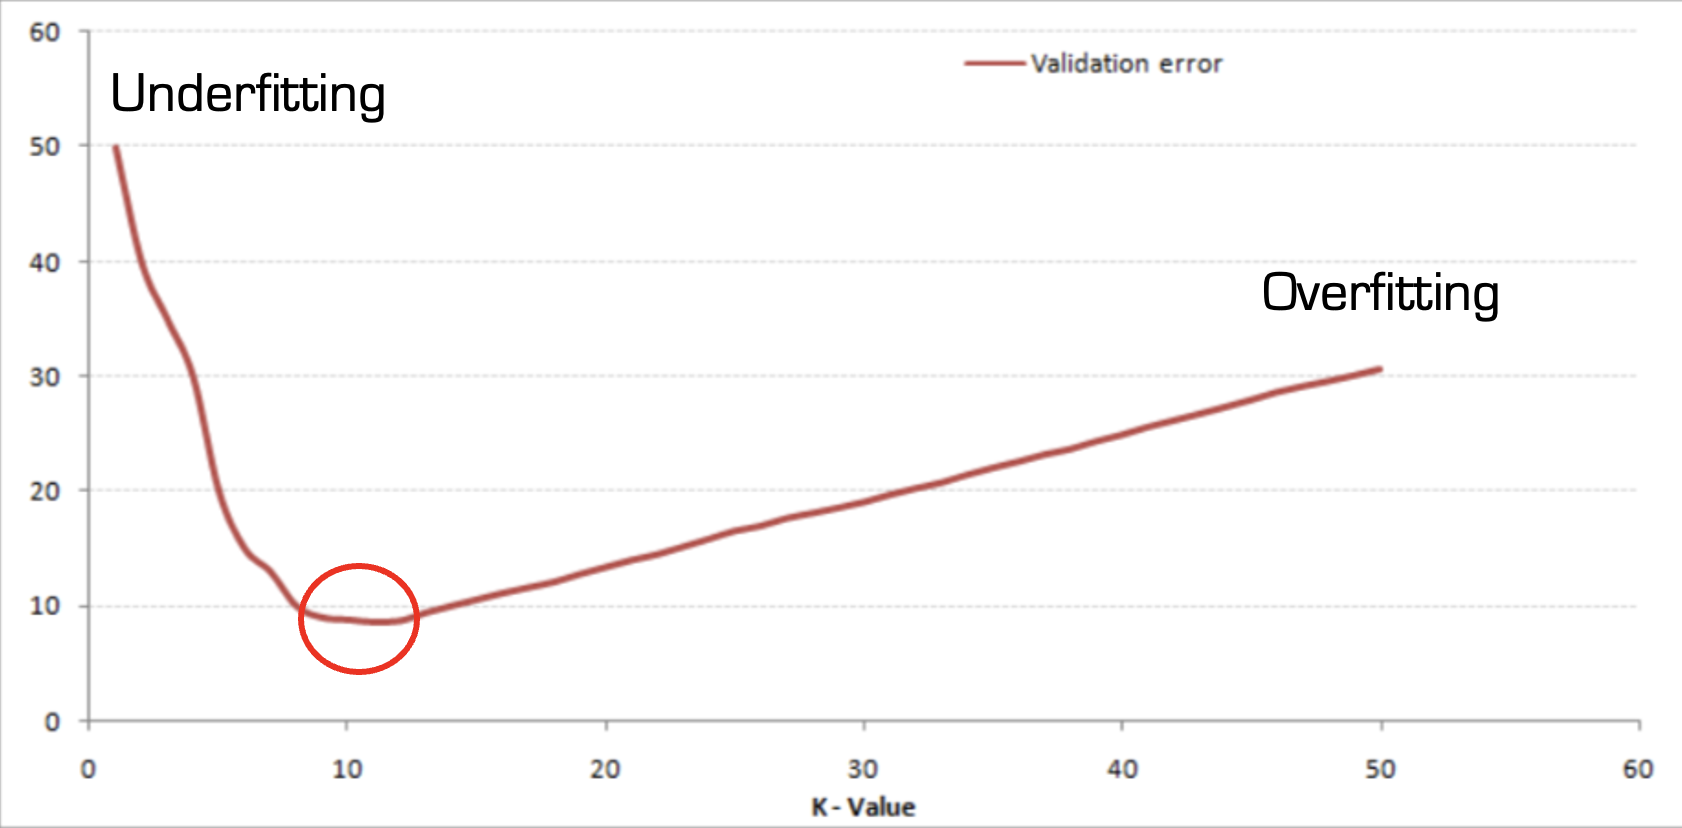
\includegraphics[width=0.6\textwidth]{images/model_selection_knn.png}
\end{center}
\end{frame}

\begin{frame}[allowframebreaks]{Classification metrics}
  Imagine you have a classification problem with two classes \textit{Sick} and \textit{Not sick}.
  
  To summarize your predictions and evaluate them, a \textit{Confusion Matrix} displays in a tabular format the numbers of true positives (predicted Sick and is Sick), true negatives (predicted Not sick and is Not sick), false positives, and false negatives.

  \begin{center}
    
    \begin{tabular}{c | c c}
      \toprule
      & \multicolumn{2}{c}{Predicted} \\
      \midrule
      Actual & A & B \\
      \midrule
      A & 85 & 15 \\
      B & 10 & 90 \\
      \bottomrule
    \end{tabular}
  \end{center}

Hence here Shown: True positives $TP = 85$, True negatives $TN = 90$  \\
False positives $FP = 10$, false negatives $FN = 15$   

From this information, we can compute a number of indicators such as 
\begin{itemize}
  \item 
 the \textbf{Accuracy}, i.e. the number of correct predictions divided by the total number of predictions made:
  $$A = \frac{TP+TN}{TP+TN+FP+FN} = \frac{85+90}{200} = 87.5 \% $$
  the \textbf{sensitivity},  i.e. the number of true positives detected divided by the total number of positive cases:
  $$S = \frac{TP}{TP+FN} = \frac{85}{85+15} = 85 \% $$
\end{itemize}


Notes: 
\begin{itemize}
  \item in this case the number of positive cases = the number of negative cases (balanced dataset); it is in general not the case and you must take care of it
  \item a confusion matrix can be generalized to a multiclass problem.
\end{itemize}

\end{frame}

\begin{frame} [allowframebreaks]{Regression metrics}\label{regression_metrics}
  Some common error metrics are the 
  \begin{itemize}
    \item \textbf{Mean absolute error}: $ MAE = \frac{1}{N}\sum_{j=1}^N| y_j - \hat{y}_j |$
    \item \textbf{Mean squared error}: $ MSE = \frac{1}{N}\sum_{j=1}^N {\left(y_j - \hat{y}_j\right)}^2$
  \end{itemize}
  They should be as small as possible. The MAE penalizes equally large and small errors, while the MSE penalizes large errors more than small errors.
  

  The \textbf{Coefficient of determination}, $R^2$, should be as close as possible to $1$, and weights errors : 
  $$R^2 = 1 - \frac{SS_{res}}{SS_{tot}}= 1 - \frac{\sum (y_i - \hat{y}_i)^2}{\sum (y_i - \bar{y})^2}$$
  Where:
  \begin{itemize}
    \item $SS_{res}$ is the sum of squares of residuals (the sum of squared errors).
    \item $SS_{tot}$ is the total sum of squares.
    \item $y_i$ are the observed values.
    \item $\hat{y}_i$ are the predicted values.
    \item $\bar{y}$ is the mean of the observed values.
  \end{itemize}

  It indicates the proportion of the variance in the dependent variable ($y$) that is predictable from the independent variable(s) ($x$)

\end{frame}

\begin{frame} {Wrap up example}

  \begin{itemize}
    \item   This code demonstrates a basic k-Nearest Neighbors (k-NN) classification using the `scikit-learn` library in Python.
    \item   It loads the Iris dataset, splits it into training and testing sets, scales the data, trains a k-NN classifier, and evaluates its accuracy.
  \end{itemize}
  \url{https://colab.research.google.com/drive/1v0BMKsY26pPStqNwEpoqOnbWTitRrB0C?usp=sharing}
  
%  \begin{lstlisting}[language=Python, breaklines=true]
%from sklearn import neighbors, datasets, preprocessing
%from sklearn.model_selection import train_test_split
%from sklearn.metrics import accuracy_score
%
%# Load the Iris dataset
%iris = datasets.load_iris()
%X, y = iris.data[:, :2], iris.target  # Use only the first two features
%
%# Split the data into training and testing sets
%X_train, X_test, y_train, y_test = train_test_split(X, y, random_state=33)
%
%# Scale the data using StandardScaler
%scaler = preprocessing.StandardScaler().fit(X_train)
%X_train = scaler.transform(X_train)
%X_test = scaler.transform(X_test)
%
%# Create a k-NN classifier with k=5
%knn = neighbors.KNeighborsClassifier(n_neighbors=5)
%
%# Train the classifier
%knn.fit(X_train, y_train)
%
%# Make predictions on the test set
%y_pred = knn.predict(X_test)
%
%# Evaluate the accuracy of the classifier
%accuracy = accuracy_score(y_test, y_pred)
%print("Accuracy:", accuracy)
%  \end{lstlisting}

\end{frame}
  


\section{Application}

\begin{frame}
  \frametitle{Fitting the power curve of a wind turbine}

  See Google Colab.
  \url{https://colab.research.google.com/drive/1UxhfjLj8UMz5EHqnYbizIXcROuo_9ItM?usp=sharing}
\end{frame}
 